% Topic T4.3: Stablecoins
% Self-contained Beamer slides for Digital Finance course
\documentclass[11pt,aspectratio=169]{beamer}
\usetheme{Madrid}

% ======================= PACKAGES =======================
\usepackage{graphicx}
\usepackage{booktabs}
\usepackage{adjustbox}
\usepackage{multicol}
\usepackage{amsmath}
\usepackage{amssymb}
\usepackage{tikz}
\usetikzlibrary{arrows,shapes,positioning,shadows,trees}
\usepackage{listings}
\usepackage{xcolor}

% ======================= COLOR DEFINITIONS =======================
% Primary color scheme: Blue/Teal for Digital Finance
\definecolor{dfblue}{RGB}{0,102,204}
\definecolor{dfteal}{RGB}{0,153,153}
\definecolor{dfcyan}{RGB}{51,187,204}
\definecolor{dflightblue}{RGB}{153,204,255}
\definecolor{dflightblue2}{RGB}{173,214,255}
\definecolor{dflightblue3}{RGB}{193,224,255}
\definecolor{dflightblue4}{RGB}{213,234,255}

% Accent colors for finance applications
\definecolor{dfgreen}{RGB}{44, 160, 44}
\definecolor{dfred}{RGB}{214, 39, 40}
\definecolor{dforange}{RGB}{255, 127, 14}
\definecolor{dfgray}{RGB}{127, 127, 127}

% Utility colors
\definecolor{lightgray}{RGB}{240, 240, 240}
\definecolor{midgray}{RGB}{180, 180, 180}
\definecolor{codebg}{RGB}{245, 245, 245}

% ======================= THEME CUSTOMIZATION =======================
% Apply Digital Finance color scheme to Madrid theme
\setbeamercolor{palette primary}{bg=dflightblue3,fg=dfblue}
\setbeamercolor{palette secondary}{bg=dflightblue2,fg=dfblue}
\setbeamercolor{palette tertiary}{bg=dfteal,fg=white}
\setbeamercolor{palette quaternary}{bg=dfblue,fg=white}

\setbeamercolor{structure}{fg=dfblue}
\setbeamercolor{section in toc}{fg=dfblue}
\setbeamercolor{subsection in toc}{fg=dfteal}
\setbeamercolor{title}{fg=dfblue}
\setbeamercolor{frametitle}{fg=dfblue,bg=dflightblue3}
\setbeamercolor{block title}{bg=dflightblue2,fg=dfblue}
\setbeamercolor{block body}{bg=dflightblue4,fg=black}

% Remove navigation symbols for cleaner look
\setbeamertemplate{navigation symbols}{}

% Clean itemize/enumerate
\setbeamertemplate{itemize items}[circle]
\setbeamertemplate{enumerate items}[default]

% Margins for readability
\setbeamersize{text margin left=8mm,text margin right=8mm}

% ======================= LISTINGS CONFIGURATION =======================
% Python code style
\lstdefinestyle{pythonstyle}{
    language=Python,
    basicstyle=\ttfamily\footnotesize,
    keywordstyle=\color{dfblue}\bfseries,
    stringstyle=\color{dforange},
    commentstyle=\color{dfgray}\itshape,
    numberstyle=\tiny\color{dfgray},
    numbers=left,
    numbersep=5pt,
    backgroundcolor=\color{codebg},
    showspaces=false,
    showstringspaces=false,
    showtabs=false,
    frame=single,
    rulecolor=\color{midgray},
    tabsize=4,
    captionpos=b,
    breaklines=true,
    breakatwhitespace=false,
    escapeinside={(*@}{@*)},
    xleftmargin=10pt,
    xrightmargin=10pt
}

% Solidity code style
\lstdefinestyle{soliditystyle}{
    language=Java, % closest approximation
    basicstyle=\ttfamily\footnotesize,
    keywordstyle=\color{dfteal}\bfseries,
    stringstyle=\color{dforange},
    commentstyle=\color{dfgray}\itshape,
    numberstyle=\tiny\color{dfgray},
    numbers=left,
    numbersep=5pt,
    backgroundcolor=\color{codebg},
    showspaces=false,
    showstringspaces=false,
    showtabs=false,
    frame=single,
    rulecolor=\color{midgray},
    tabsize=2,
    captionpos=b,
    breaklines=true,
    breakatwhitespace=false,
    escapeinside={(*@}{@*)},
    xleftmargin=10pt,
    xrightmargin=10pt,
    morekeywords={pragma, contract, function, returns, public, private, view, pure, payable, address, uint256, mapping, event, modifier}
}

% Inline code command
\newcommand{\code}[1]{\texttt{\color{dfblue}#1}}

% ======================= CUSTOM COMMANDS =======================
% Bottom annotation (Madrid-style)
\newcommand{\bottomnote}[1]{%
\vfill
\vspace{-2mm}
\textcolor{dflightblue2}{\rule{\textwidth}{0.4pt}}
\vspace{1mm}
\footnotesize
\textbf{#1}
}

% Compact list spacing
\newcommand{\compactlist}{%
\setlength{\itemsep}{0pt}%
\setlength{\parskip}{0pt}%
\setlength{\parsep}{0pt}%
}

% Chart placeholder
\newcommand{\chartplaceholder}[2][5cm]{%
\begin{center}
\begin{adjustbox}{max width=0.95\textwidth, max height=#1}
\framebox[\textwidth][c]{%
\rule{0pt}{#1}%
\textcolor{midgray}{[#2]}%
}
\end{adjustbox}
\end{center}
}

% ======================= FINANCE NOTATION MACROS =======================
% Probability and statistics
\newcommand{\E}{\mathbb{E}} % Expected value
\newcommand{\Var}{\mathrm{Var}} % Variance
\newcommand{\Cov}{\mathrm{Cov}} % Covariance
\newcommand{\Prob}{\mathbb{P}} % Probability

% Distributions
\newcommand{\Normal}{\mathcal{N}} % Normal distribution
\newcommand{\Uniform}{\mathcal{U}} % Uniform distribution

% Returns and prices
\newcommand{\Ret}{R} % Return
\newcommand{\LogRet}{r} % Log return
\newcommand{\Price}{S} % Price/Stock price
\newcommand{\Strike}{K} % Strike price

% Options and derivatives
\newcommand{\CallPrice}{C} % Call option price
\newcommand{\PutPrice}{P} % Put option price
\newcommand{\Greeks}[1]{\mathit{#1}} % Greek letters

% Risk measures
\newcommand{\VaR}{\mathrm{VaR}} % Value at Risk
\newcommand{\CVaR}{\mathrm{CVaR}} % Conditional VaR
\newcommand{\Sharpe}{\mathrm{SR}} % Sharpe Ratio

% Time series
\newcommand{\AR}{\mathrm{AR}} % Autoregressive
\newcommand{\MA}{\mathrm{MA}} % Moving average
\newcommand{\GARCH}{\mathrm{GARCH}} % GARCH

% Blockchain/Crypto
\newcommand{\Hash}{\mathrm{Hash}} % Hash function
\newcommand{\Block}{\mathcal{B}} % Block
\newcommand{\Chain}{\mathcal{C}} % Chain

% Real numbers, integers
\newcommand{\R}{\mathbb{R}}
\newcommand{\Z}{\mathbb{Z}}
\newcommand{\N}{\mathbb{N}}

% ======================= TIKZ STYLES =======================
% Styles for finance-related diagrams
\tikzstyle{process} = [rectangle, minimum width=3cm, minimum height=1cm, text centered, draw=dfblue, fill=dflightblue4, thick]
\tikzstyle{decision} = [diamond, minimum width=3cm, minimum height=1cm, text centered, draw=dfteal, fill=dflightblue4, thick]
\tikzstyle{arrow} = [thick,->,>=stealth,color=dfblue]
\tikzstyle{blockchain} = [rectangle, rounded corners, minimum width=2.5cm, minimum height=1cm, text centered, draw=dfteal, fill=dflightblue3, thick]
\tikzstyle{transaction} = [circle, minimum size=0.8cm, text centered, draw=dforange, fill=dflightblue4, thick]

% ======================= FOOTER TEMPLATE =======================
\setbeamertemplate{footline}{
    \hbox{\begin{beamercolorbox}[wd=\paperwidth,ht=2.5ex,dp=1ex,leftskip=.5em,rightskip=.5em]{author in head/foot}
    \tiny
    \textbf{Digital Finance} \hfill
    Joerg Osterrieder \hfill
    \insertdate \hfill
    Page \insertframenumber{} / \inserttotalframenumber
    \end{beamercolorbox}}
}

% ======================= SECTION DIVIDER TEMPLATE =======================
\AtBeginSection[]{
\begin{frame}[plain]
\vfill
\centering
\begin{beamercolorbox}[sep=12pt,center]{title}
\usebeamerfont{title}\LARGE\insertsection\par
\end{beamercolorbox}
\vfill
\end{frame}
}


\title[T4.3: Stablecoins]{Topic 4.3: Stablecoins}
\subtitle{The Bridge Between Crypto and Fiat}
\author{Joerg Osterrieder}
\institute{Digital Finance}
\date{2025}

\begin{document}

% =============================================================================
% Frame 1: Title Slide
% =============================================================================
\begin{frame}[plain]
\titlepage
\end{frame}

% =============================================================================
% Frame 2: Learning Objectives
% =============================================================================
\begin{frame}{Learning Objectives}
\begin{center}
\textbf{\Large What You Will Learn in This Topic}
\end{center}

\vspace{5mm}
By the end of this session, you will be able to:

\begin{enumerate}
\item \textbf{Classify} stablecoins by design type (fiat-backed, crypto-collateralized, algorithmic)
\item \textbf{Explain} the mechanisms that maintain price stability for each type
\item \textbf{Assess} de-peg risk factors and analyze historical de-peg events
\item \textbf{Understand} the Stablecoin Trilemma and its design implications
\item \textbf{Articulate} why stablecoins face heavy regulatory scrutiny
\end{enumerate}

\vspace{5mm}
\begin{block}{Hands-On Component}
NB10: Analyze stablecoin price stability data---examine de-peg events and compare resilience across designs.
\end{block}
\end{frame}

% =============================================================================
% Frame 3: Prerequisites/Background I
% =============================================================================
\begin{frame}{Prerequisites: Why Price Stability Matters}
\begin{columns}[T]
\begin{column}{0.48\textwidth}
\textbf{The Volatility Problem:}
\begin{itemize}
\item Bitcoin: 60\%+ annual volatility
\item Unsuitable for everyday payments
\item Merchant pricing becomes impossible
\item DeFi needs stable base assets
\end{itemize}

\vspace{3mm}
\textbf{Prior Knowledge Required:}
\begin{itemize}
\item Basic understanding of cryptocurrency
\item DeFi primitives (T4.2)
\item Smart contracts (T4.1)
\end{itemize}
\end{column}
\begin{column}{0.48\textwidth}
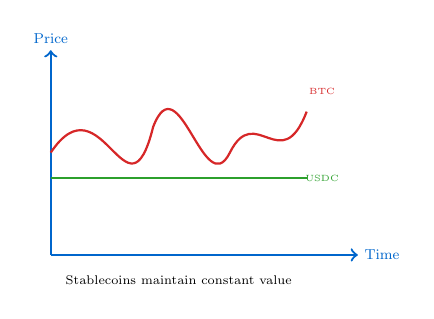
\begin{tikzpicture}[scale=0.65, transform shape]
% Volatility comparison
\draw[thick, dfblue, ->] (0,0) -- (6,0) node[right] {\footnotesize Time};
\draw[thick, dfblue, ->] (0,0) -- (0,4) node[above] {\footnotesize Price};

% BTC volatile line
\draw[thick, dfred] (0,2)
    .. controls (1,3.5) and (1.5,0.5) .. (2,2.5)
    .. controls (2.5,3.8) and (3,1) .. (3.5,2)
    .. controls (4,3) and (4.5,1.5) .. (5,2.8);
\node[dfred, font=\tiny] at (5.3,3.2) {BTC};

% Stablecoin flat line
\draw[thick, dfgreen] (0,1.5) -- (5,1.5);
\node[dfgreen, font=\tiny] at (5.3,1.5) {USDC};

% Label
\node[font=\scriptsize] at (2.5,-0.5) {Stablecoins maintain constant value};
\end{tikzpicture}

\vspace{3mm}
\begin{alertblock}{Key Insight}
Stablecoins bridge TradFi and crypto by providing price predictability in a volatile ecosystem.
\end{alertblock}
\end{column}
\end{columns}
\end{frame}

% =============================================================================
% Frame 4: Prerequisites/Background II
% =============================================================================
\begin{frame}{The Problem Stablecoins Solve}
\begin{center}
\textbf{\Large On-Chain ``Cash'' for the Crypto Economy}
\end{center}

\vspace{3mm}
\begin{columns}[T]
\begin{column}{0.48\textwidth}
\textbf{Without Stablecoins:}
\begin{itemize}
\item Trading requires moving to fiat
\item DeFi cannot price loans reliably
\item Cross-border payments face friction
\item No on-chain savings in stable value
\end{itemize}

\vspace{3mm}
\textbf{Market Size (2024):}
\begin{itemize}
\item Total supply: \$170B+
\item Daily volume: \$50B+
\item Surpasses Visa in some metrics
\end{itemize}
\end{column}
\begin{column}{0.48\textwidth}
\textbf{Use Cases:}
\begin{itemize}
\item \textbf{Trading pairs} on exchanges
\item \textbf{DeFi collateral} and lending
\item \textbf{Remittances} (24/7, low fees)
\item \textbf{Savings} in dollarized economies
\item \textbf{Payroll} and B2B payments
\end{itemize}

\vspace{3mm}
\begin{block}{Why \$1 Peg?}
USD is the global reserve currency. A dollar-pegged stablecoin inherits this network effect.
\end{block}
\end{column}
\end{columns}
\end{frame}

% =============================================================================
% Frame 5: Definition and Overview
% =============================================================================
\begin{frame}{What Are Stablecoins?}
\begin{columns}[T]
\begin{column}{0.55\textwidth}
\begin{block}{Definition}
\textbf{Stablecoins} are cryptocurrencies designed to maintain a stable value relative to a reference asset (typically USD).
\end{block}

\vspace{0.3cm}
\textbf{Core Challenge:}
\begin{itemize}
\item How do you maintain \$1 value without a central bank?
\item Three fundamentally different approaches exist
\item Each involves different trust assumptions
\item No perfect solution---only trade-offs
\end{itemize}
\end{column}

\begin{column}{0.42\textwidth}
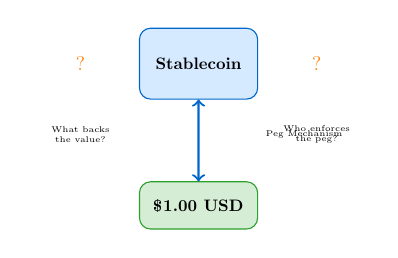
\begin{tikzpicture}[scale=0.6, transform shape]
% Peg illustration
\node[rectangle, draw=dfblue, fill=dflightblue4, minimum width=2.5cm, minimum height=1.5cm, rounded corners] (stable) at (0,2) {\textbf{Stablecoin}};
\node[rectangle, draw=dfgreen, fill=dfgreen!20, minimum width=2.5cm, minimum height=1cm, rounded corners] (dollar) at (0,-1) {\textbf{\$1.00 USD}};

% Peg connection
\draw[thick, dfblue, <->] (stable) -- (dollar);
\node[right, font=\tiny] at (1.3,0.5) {Peg Mechanism};

% Question marks around
\node[font=\large, dforange] at (-2.5,2) {?};
\node[font=\large, dforange] at (2.5,2) {?};
\node[font=\tiny, text width=2cm, align=center] at (-2.5,0.5) {What backs the value?};
\node[font=\tiny, text width=2cm, align=center] at (2.5,0.5) {Who enforces the peg?};
\end{tikzpicture}
\end{column}
\end{columns}

\vspace{3mm}
\begin{alertblock}{The Central Question}
How do you create ``digital dollars'' that maintain purchasing power without the Federal Reserve?
\end{alertblock}
\end{frame}

% =============================================================================
% Frame 6: Stablecoin Design Taxonomy
% =============================================================================
\begin{frame}{Stablecoin Design Taxonomy}
\begin{center}
\begin{tikzpicture}[scale=0.7, transform shape]
    % Root
    \node[smartcontract, minimum width=3cm, fill=dfblue!30] (root) at (0, 3) {Stablecoins};

    % Three types
    \node[smartcontract, minimum width=2.5cm, fill=dfgreen!30] (fiat) at (-5, 0.5) {Fiat-Backed};
    \node[smartcontract, minimum width=2.5cm, fill=dforange!30] (crypto) at (0, 0.5) {Crypto-Collateralized};
    \node[smartcontract, minimum width=2.5cm, fill=dfred!30] (algo) at (5, 0.5) {Algorithmic};

    % Examples
    \node[font=\scriptsize] at (-5, -0.7) {USDT, USDC};
    \node[font=\scriptsize] at (-5, -1.2) {PYUSD, EURC};

    \node[font=\scriptsize] at (0, -0.7) {DAI, LUSD};
    \node[font=\scriptsize] at (0, -1.2) {sUSD};

    \node[font=\scriptsize] at (5, -0.7) {FRAX (hybrid)};
    \node[font=\scriptsize] at (5, -1.2) {\sout{UST} (failed)};

    % Arrows
    \draw[arrow] (root) -- (fiat);
    \draw[arrow] (root) -- (crypto);
    \draw[arrow] (root) -- (algo);

    % Trust spectrum
    \draw[arrow, line width=2pt] (-6, -2.5) -- (6, -2.5);
    \node[font=\small] at (-5, -3) {More Trust};
    \node[font=\small] at (5, -3) {Less Trust};
    \node[font=\small] at (0, -3) {Required};
\end{tikzpicture}
\end{center}

\vspace{3mm}
\textbf{Key Insight:} Each design trades off between decentralization, capital efficiency, and stability.
\end{frame}

% =============================================================================
% Frame 7: Fiat-Backed Stablecoins - Overview
% =============================================================================
\begin{frame}{Fiat-Backed Stablecoins: How They Work}
\begin{columns}[T]
\begin{column}{0.48\textwidth}
\textbf{Mechanism:}
\begin{enumerate}
\item User sends \$1 to issuer
\item Issuer holds \$1 in reserves
\item Issuer mints 1 stablecoin
\item User can redeem anytime
\end{enumerate}

\vspace{0.3cm}
\textbf{Examples:}
\begin{itemize}
\item \textbf{USDT} (Tether): \$110B, largest
\item \textbf{USDC} (Circle): \$35B, regulated
\item \textbf{PYUSD} (PayPal): Newest entrant
\end{itemize}
\end{column}

\begin{column}{0.48\textwidth}
\begin{tikzpicture}[scale=0.6, transform shape]
    % Bank
    \node[rectangle, draw=dfblue, fill=dflightblue4, minimum width=2.5cm, minimum height=2cm, rounded corners] (bank) at (0, 0) {};
    \node[font=\small\bfseries] at (0, 0.5) {Reserve};
    \node[font=\scriptsize] at (0, -0.1) {\$100M USD};
    \node[font=\tiny] at (0, -0.6) {(audited)};

    % Issuer
    \node[smartcontract, minimum width=2cm] (issuer) at (0, 3) {Issuer};

    % Supply
    \node[rectangle, draw=dforange, fill=dforange!20, minimum width=2.5cm, minimum height=1cm, rounded corners] (supply) at (4, 0) {100M USDC};

    % Arrows
    \draw[arrow] (issuer) -- (bank) node[midway, left, font=\tiny] {Deposits};
    \draw[arrow] (issuer) -- (supply) node[midway, above, font=\tiny] {Mints};
\end{tikzpicture}

\vspace{0.3cm}
\textbf{Peg Maintenance:}
\begin{itemize}
\item Arbitrage keeps price at \$1
\item If price $>$ \$1: mint and sell
\item If price $<$ \$1: buy and redeem
\end{itemize}
\end{column}
\end{columns}
\end{frame}

% =============================================================================
% Frame 8: Fiat-Backed Stablecoins - Risks
% =============================================================================
\begin{frame}{Fiat-Backed Stablecoins: Trust Requirements}
\begin{columns}[T]
\begin{column}{0.48\textwidth}
\textbf{What You Must Trust:}
\begin{itemize}
\item Issuer holds stated reserves
\item Reserves are liquid and accessible
\item Issuer won't be hacked or defrauded
\item Issuer will honor redemptions
\item Banking partners remain stable
\end{itemize}

\vspace{3mm}
\textbf{USDT Reserve Composition:}
\begin{itemize}
\item Cash \& equivalents: 85\%+
\item Corporate bonds: small \%
\item Secured loans: small \%
\item Other investments: small \%
\end{itemize}
\end{column}

\begin{column}{0.48\textwidth}
\begin{alertblock}{Centralization Risks}
\begin{itemize}
\item Can freeze/blacklist addresses
\item Regulatory seizure possible
\item Single point of failure
\item Opaque reserve reporting (USDT)
\end{itemize}
\end{alertblock}

\vspace{3mm}
\textbf{USDC vs USDT:}
\begin{itemize}
\item USDC: Monthly attestations, regulated
\item USDT: Less transparent, offshore
\item Both: Centralized freeze capability
\end{itemize}
\end{column}
\end{columns}

\vspace{3mm}
\begin{block}{Key Trade-off}
Fiat-backing provides strong stability but reintroduces the centralization that crypto was designed to avoid.
\end{block}
\end{frame}

% =============================================================================
% Frame 9: Crypto-Collateralized Stablecoins - Overview
% =============================================================================
\begin{frame}{Crypto-Collateralized Stablecoins}
\begin{columns}[T]
\begin{column}{0.48\textwidth}
\textbf{How It Works:}
\begin{enumerate}
\item User deposits \$150 ETH
\item Protocol mints 100 DAI
\item Collateral ratio: 150\%
\item If ETH drops, liquidation
\end{enumerate}

\vspace{0.3cm}
\textbf{MakerDAO/DAI:}
\begin{itemize}
\item Decentralized governance
\item Multiple collateral types
\item Stability fee (interest)
\item Liquidation at 150\%
\end{itemize}
\end{column}

\begin{column}{0.48\textwidth}
\begin{tikzpicture}[scale=0.55, transform shape]
    % Vault
    \node[rectangle, draw=dfblue, fill=dflightblue3, minimum width=3cm, minimum height=3cm, rounded corners] (vault) at (0, 0) {};
    \node[font=\small\bfseries] at (0, 0.9) {CDP/Vault};
    \node[font=\scriptsize] at (0, 0.2) {\$150 ETH};
    \node[font=\tiny] at (0, -0.3) {(locked)};

    % User
    \node[smartcontract] (user) at (-4, 0) {User};

    % DAI
    \node[rectangle, draw=dforange, fill=dforange!20, minimum width=2cm, minimum height=0.8cm, rounded corners] (dai) at (4, 0) {100 DAI};

    % Arrows
    \draw[arrow] (user) -- (-1.5, 0) node[midway, above, font=\tiny] {Lock ETH};
    \draw[arrow] (1.5, 0) -- (dai) node[midway, above, font=\tiny] {Mint};

    % Collateral ratio
    \node[rectangle, draw=dfgreen, fill=dfgreen!20, rounded corners, font=\scriptsize] at (0, -2) {150\% Collateralized};
\end{tikzpicture}

\vspace{0.2cm}
\textbf{Why Over-Collateralization?}
\begin{itemize}
\item Crypto collateral is volatile
\item 150\% provides safety buffer
\item Liquidation protects the peg
\end{itemize}
\end{column}
\end{columns}
\end{frame}

% =============================================================================
% Frame 10: Crypto-Collateralized - Liquidation Mechanics
% =============================================================================
\begin{frame}{Liquidation Mechanics}
\begin{center}
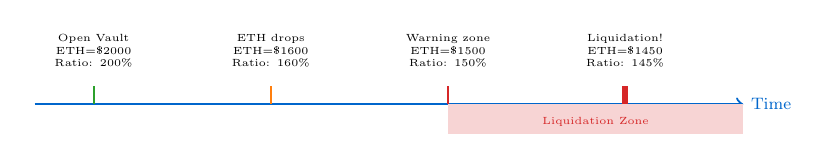
\begin{tikzpicture}[scale=0.75, transform shape]
% Timeline
\draw[thick, dfblue, ->] (0,0) -- (12,0) node[right] {\footnotesize Time};

% Events
\node[above, text width=2cm, align=center, font=\tiny] at (1,0.5) {Open Vault\\ETH=\$2000\\Ratio: 200\%};
\draw[thick, dfgreen] (1,0) -- (1,0.3);

\node[above, text width=2cm, align=center, font=\tiny] at (4,0.5) {ETH drops\\ETH=\$1600\\Ratio: 160\%};
\draw[thick, dforange] (4,0) -- (4,0.3);

\node[above, text width=2cm, align=center, font=\tiny] at (7,0.5) {Warning zone\\ETH=\$1500\\Ratio: 150\%};
\draw[thick, dfred] (7,0) -- (7,0.3);

\node[above, text width=2.5cm, align=center, font=\tiny] at (10,0.5) {Liquidation!\\ETH=\$1450\\Ratio: 145\%};
\draw[thick, dfred, line width=2pt] (10,0) -- (10,0.3);

% Danger zone shading
\draw[fill=dfred!20, draw=none] (7,-0.5) rectangle (12,0);
\node[font=\tiny, dfred] at (9.5,-0.3) {Liquidation Zone};
\end{tikzpicture}
\end{center}

\vspace{3mm}
\textbf{Liquidation Process:}
\begin{enumerate}
\item Collateral ratio falls below threshold (e.g., 150\%)
\item Anyone can trigger liquidation via smart contract
\item Collateral sold at discount (liquidation penalty: 13\%)
\item Debt repaid, remainder returned to vault owner
\end{enumerate}

\vspace{3mm}
\begin{alertblock}{Liquidation Cascades}
During market crashes, mass liquidations can cause collateral fire sales, pushing prices lower, triggering more liquidations---a dangerous feedback loop.
\end{alertblock}
\end{frame}

% =============================================================================
% Frame 11: Crypto-Collateralized Trade-offs
% =============================================================================
\begin{frame}{Crypto-Collateralized: Trade-offs}
\begin{columns}[T]
\begin{column}{0.48\textwidth}
\textbf{Advantages:}
\begin{itemize}
\item[\textcolor{dfgreen}{\checkmark}] \textbf{Decentralized}---no single issuer
\item[\textcolor{dfgreen}{\checkmark}] \textbf{Transparent}---on-chain reserves
\item[\textcolor{dfgreen}{\checkmark}] \textbf{Censorship-resistant}
\item[\textcolor{dfgreen}{\checkmark}] \textbf{No counterparty risk}
\item[\textcolor{dfgreen}{\checkmark}] \textbf{Auditable in real-time}
\end{itemize}

\vspace{3mm}
\textbf{Example Protocols:}
\begin{itemize}
\item DAI (MakerDAO)
\item LUSD (Liquity)
\item sUSD (Synthetix)
\end{itemize}
\end{column}

\begin{column}{0.48\textwidth}
\textbf{Disadvantages:}
\begin{itemize}
\item[\textcolor{dfred}{$\times$}] \textbf{Capital inefficient}---need \$150 for \$100
\item[\textcolor{dfred}{$\times$}] \textbf{Liquidation risk} for users
\item[\textcolor{dfred}{$\times$}] \textbf{Complex} for average users
\item[\textcolor{dfred}{$\times$}] \textbf{Smart contract risk}
\item[\textcolor{dfred}{$\times$}] \textbf{Scalability limited} by collateral
\end{itemize}

\vspace{3mm}
\begin{block}{Capital Efficiency}
To mint \$1B in DAI requires \$1.5B+ in collateral locked up, making it less scalable than fiat-backed alternatives.
\end{block}
\end{column}
\end{columns}
\end{frame}

% =============================================================================
% Frame 12: Algorithmic Stablecoins - Overview
% =============================================================================
\begin{frame}{Algorithmic Stablecoins: The Experiment}
\begin{columns}[T]
\begin{column}{0.48\textwidth}
\textbf{Pure Algorithmic (Failed):}
\begin{itemize}
\item No collateral backing
\item Dual-token: stable + governance
\item Expand supply when above peg
\item Contract supply when below peg
\end{itemize}

\vspace{0.2cm}
\textbf{The Death Spiral:}
\begin{enumerate}
\item Price drops below peg
\item Redemptions spike
\item Confidence collapses
\item Governance token crashes
\item System becomes insolvent
\end{enumerate}
\end{column}

\begin{column}{0.48\textwidth}
\begin{alertblock}{Case Study: UST/LUNA (May 2022)}
\begin{itemize}
\item Peak market cap: \$18B
\item Collapsed in 72 hours
\item \$60B total value destroyed
\item Triggered crypto contagion
\end{itemize}
\end{alertblock}

\vspace{0.3cm}
\textbf{Hybrid Models (Surviving):}
\begin{itemize}
\item \textbf{FRAX}: Partially collateralized
\item Dynamic collateral ratio
\item More resilient to de-peg
\end{itemize}
\end{column}
\end{columns}
\end{frame}

% =============================================================================
% Frame 13: Terra/UST Collapse Explained
% =============================================================================
\begin{frame}{Case Study: Terra/UST Collapse}
\begin{center}
\begin{tikzpicture}[scale=0.7, transform shape]
% Death spiral visualization
\node[smartcontract, minimum width=2.5cm, fill=dflightblue3] (ust) at (0,3) {UST Price Drops};
\node[smartcontract, minimum width=2.5cm, fill=dflightblue2] (redeem) at (4,1.5) {Users Redeem UST};
\node[smartcontract, minimum width=2.5cm, fill=dforange!30] (mint) at (4,-1.5) {LUNA Minted};
\node[smartcontract, minimum width=2.5cm, fill=dfred!30] (luna) at (0,-3) {LUNA Price Crashes};
\node[smartcontract, minimum width=2.5cm, fill=dfred!50] (confidence) at (-4,-1.5) {Confidence Collapses};
\node[smartcontract, minimum width=2.5cm, fill=dfred!30] (more) at (-4,1.5) {More Selling};

% Arrows forming cycle
\draw[arrow, thick] (ust) -- (redeem);
\draw[arrow, thick] (redeem) -- (mint);
\draw[arrow, thick] (mint) -- (luna);
\draw[arrow, thick] (luna) -- (confidence);
\draw[arrow, thick] (confidence) -- (more);
\draw[arrow, thick] (more) -- (ust);

% Center label
\node[font=\large\bfseries, dfred] at (0,0) {DEATH SPIRAL};
\end{tikzpicture}
\end{center}

\vspace{3mm}
\textbf{Key Lesson:} When the peg mechanism relies on a token whose value depends on confidence in the peg, you create a reflexive loop that can collapse catastrophically.
\end{frame}

% =============================================================================
% Frame 14: Algorithmic Stablecoin Mechanics
% =============================================================================
\begin{frame}{Algorithmic Mechanism: Mint/Burn}
\begin{columns}[T]
\begin{column}{0.48\textwidth}
\textbf{Above Peg (\$1.02):}
\begin{enumerate}
\item Arbitrageurs mint new stablecoins
\item Pay \$1 worth of governance token
\item Sell stablecoin for \$1.02
\item Profit: \$0.02 per coin
\item Increased supply pushes price down
\end{enumerate}

\vspace{3mm}
\textbf{This direction works well.}
\end{column}

\begin{column}{0.48\textwidth}
\textbf{Below Peg (\$0.98):}
\begin{enumerate}
\item Arbitrageurs buy stablecoin at \$0.98
\item Redeem for \$1 worth of governance token
\item Sell governance token
\item \textcolor{dfred}{But who buys the governance token?}
\item \textcolor{dfred}{Selling pressure crashes it}
\end{enumerate}

\vspace{3mm}
\textbf{This direction is fragile.}
\end{column}
\end{columns}

\vspace{5mm}
\begin{alertblock}{The Fundamental Problem}
Algorithmic stability depends on \textit{someone} absorbing losses during de-peg events. Without real collateral, this relies purely on confidence---which can evaporate instantly.
\end{alertblock}
\end{frame}

% =============================================================================
% Frame 15: Stablecoin Design Comparison
% =============================================================================
\begin{frame}{Stablecoin Design Comparison}
\begin{center}
\footnotesize
\begin{tabular}{p{2.5cm}|p{3.2cm}|p{3.2cm}|p{3.2cm}}
\toprule
\textbf{Attribute} & \textbf{Fiat-Backed} & \textbf{Crypto-Collateral} & \textbf{Algorithmic} \\
\midrule
Collateral & Fiat in bank & Crypto (150\%+) & None/Partial \\
Centralization & High & Medium & Low \\
Capital Efficiency & High (1:1) & Low (over-collateral) & High (0 collateral) \\
Scalability & Limited by reserves & Limited by collateral & Theoretically unlimited \\
Peg Stability & Strong & Strong & Weak \\
Regulatory Risk & High & Medium & Low \\
Censorship Risk & High & Low & Very Low \\
\bottomrule
\end{tabular}
\end{center}

\vspace{0.3cm}
\begin{block}{The Stablecoin Trilemma}
\begin{center}
You can optimize for two of three: \textbf{Decentralization}, \textbf{Stability}, \textbf{Capital Efficiency}
\end{center}
\end{block}
\end{frame}

% =============================================================================
% Frame 16: The Stablecoin Trilemma Visualized
% =============================================================================
\begin{frame}{The Stablecoin Trilemma}
\begin{center}
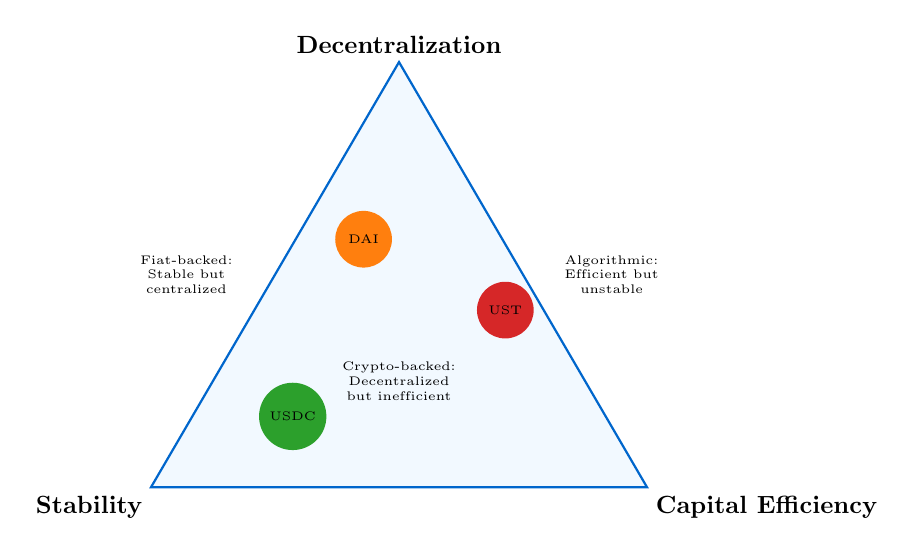
\begin{tikzpicture}[scale=0.9, transform shape]
% Triangle
\coordinate (D) at (0,4);
\coordinate (S) at (-3.5,-2);
\coordinate (C) at (3.5,-2);

\draw[thick, dfblue, fill=dflightblue4!30] (D) -- (S) -- (C) -- cycle;

% Labels
\node[above, font=\bfseries] at (D) {Decentralization};
\node[below left, font=\bfseries] at (S) {Stability};
\node[below right, font=\bfseries] at (C) {Capital Efficiency};

% Position stablecoins
\node[circle, fill=dfgreen, minimum size=0.8cm, font=\tiny] (usdc) at (-1.5, -1) {USDC};
\node[circle, fill=dforange, minimum size=0.8cm, font=\tiny] (dai) at (-0.5, 1.5) {DAI};
\node[circle, fill=dfred, minimum size=0.8cm, font=\tiny] (ust) at (1.5, 0.5) {UST};

% Annotations
\node[font=\tiny, text width=2cm, align=center] at (-3, 1) {Fiat-backed:\\Stable but\\centralized};
\node[font=\tiny, text width=2cm, align=center] at (0, -0.5) {Crypto-backed:\\Decentralized\\but inefficient};
\node[font=\tiny, text width=2cm, align=center] at (3, 1) {Algorithmic:\\Efficient but\\unstable};
\end{tikzpicture}
\end{center}

\vspace{3mm}
\textbf{No stablecoin achieves all three.} Design choices reflect priorities.
\end{frame}

% =============================================================================
% Frame 17: De-Peg Events Historical Analysis
% =============================================================================
\begin{frame}{De-Peg Events: Historical Analysis}
\begin{center}
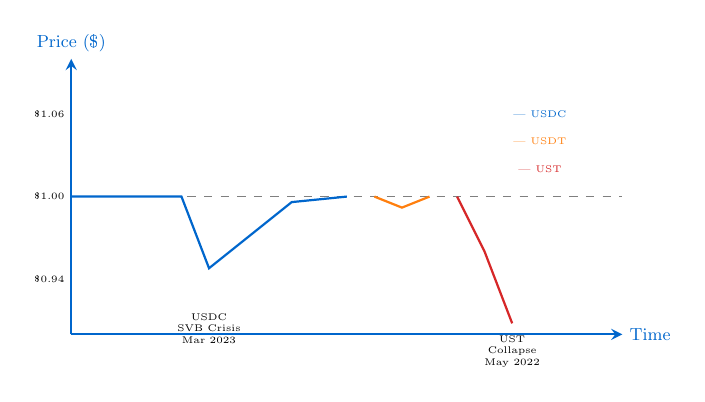
\begin{tikzpicture}[scale=0.7, transform shape]
    % Axes
    \draw[arrow] (0,0) -- (10,0) node[right, font=\small] {Time};
    \draw[arrow] (0,0) -- (0,5) node[above, font=\small] {Price (\$)};

    % Reference line at $1
    \draw[dashed, dfgray] (0, 2.5) -- (10, 2.5);
    \node[left, font=\tiny] at (0, 2.5) {\$1.00};
    \node[left, font=\tiny] at (0, 4) {\$1.06};
    \node[left, font=\tiny] at (0, 1) {\$0.94};

    % USDC de-peg (March 2023)
    \draw[thick, dfblue] (0, 2.5) -- (2, 2.5) -- (2.5, 1.2) -- (4, 2.4) -- (5, 2.5);
    \node[below, font=\tiny, text width=2cm, align=center] at (2.5, 0.5) {USDC\\SVB Crisis\\Mar 2023};

    % USDT de-peg
    \draw[thick, dforange] (5.5, 2.5) -- (6, 2.3) -- (6.5, 2.5);

    % UST collapse
    \draw[thick, dfred] (7, 2.5) -- (7.5, 1.5) -- (8, 0.2);
    \node[below, font=\tiny, text width=2cm, align=center] at (8, 0.1) {UST\\Collapse\\May 2022};

    % Legend
    \node[font=\tiny, dfblue] at (8.5, 4) {--- USDC};
    \node[font=\tiny, dforange] at (8.5, 3.5) {--- USDT};
    \node[font=\tiny, dfred] at (8.5, 3) {--- UST};
\end{tikzpicture}
\end{center}

\textbf{Key Lessons:}
\begin{itemize}
\item Fiat-backed: Banking system dependencies (SVB, Silvergate)
\item Algorithmic: Fundamental design flaws lead to death spirals
\item All designs: Confidence is fragile and self-reinforcing
\end{itemize}
\end{frame}

% =============================================================================
% Frame 18: USDC SVB Crisis Deep Dive
% =============================================================================
\begin{frame}{Case Study: USDC and Silicon Valley Bank}
\begin{columns}[T]
\begin{column}{0.48\textwidth}
\textbf{March 2023 Crisis:}
\begin{enumerate}
\item SVB bank run announced (Mar 9)
\item Circle disclosed \$3.3B in SVB
\item USDC fell to \$0.87 (Mar 11)
\item Fed backstop announced (Mar 12)
\item USDC recovered to \$1.00
\end{enumerate}

\vspace{3mm}
\textbf{Key Numbers:}
\begin{itemize}
\item Total USDC supply: \$43B
\item SVB exposure: \$3.3B (7.7\%)
\item Maximum de-peg: 13\%
\item Recovery time: 48 hours
\end{itemize}
\end{column}

\begin{column}{0.48\textwidth}
\begin{alertblock}{Lessons Learned}
\begin{itemize}
\item Fiat-backed $\neq$ risk-free
\item Banking concentration is risky
\item Government backstop saved USDC
\item Decentralized alternatives gained attention
\end{itemize}
\end{alertblock}

\vspace{3mm}
\textbf{Circle's Response:}
\begin{itemize}
\item Diversified banking partners
\item Increased T-bill holdings
\item More frequent attestations
\end{itemize}
\end{column}
\end{columns}
\end{frame}

% =============================================================================
% Frame 19: Peg Deviation Metrics
% =============================================================================
\begin{frame}{Measuring Stablecoin Stability}
\begin{columns}[T]
\begin{column}{0.48\textwidth}
\textbf{Key Metrics:}
\begin{itemize}
\item \textbf{Mean deviation}: Average distance from \$1
\item \textbf{Max deviation}: Worst-case de-peg
\item \textbf{Time in band}: \% of time within $\pm$1\%
\item \textbf{Volatility}: Standard deviation of price
\item \textbf{Recovery time}: Hours to return to peg
\end{itemize}

\vspace{3mm}
\textbf{Typical Performance:}
\begin{itemize}
\item USDC: $\pm$0.1\% (99\% of time)
\item DAI: $\pm$0.5\% (95\% of time)
\item Algorithmic: $\pm$2\%+ (variable)
\end{itemize}
\end{column}

\begin{column}{0.48\textwidth}
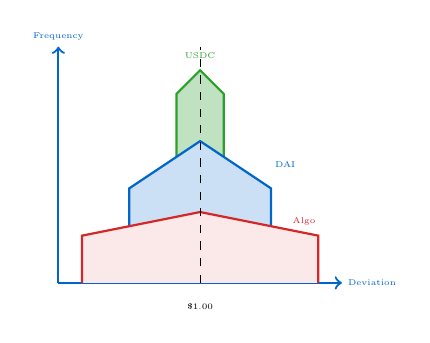
\begin{tikzpicture}[scale=0.6, transform shape]
% Histogram-like visualization
\draw[thick, dfblue, ->] (0,0) -- (6,0) node[right] {\tiny Deviation};
\draw[thick, dfblue, ->] (0,0) -- (0,5) node[above] {\tiny Frequency};

% USDC - tight distribution
\draw[thick, dfgreen, fill=dfgreen!30] (2.5,0) -- (2.5,4) -- (3,4.5) -- (3.5,4) -- (3.5,0);
\node[font=\tiny, dfgreen] at (3,4.8) {USDC};

% DAI - medium distribution
\draw[thick, dfblue, fill=dfblue!20] (1.5,0) -- (1.5,2) -- (3,3) -- (4.5,2) -- (4.5,0);
\node[font=\tiny, dfblue] at (4.8,2.5) {DAI};

% Algorithmic - wide distribution
\draw[thick, dfred, fill=dfred!10] (0.5,0) -- (0.5,1) -- (3,1.5) -- (5.5,1) -- (5.5,0);
\node[font=\tiny, dfred] at (5.2,1.3) {Algo};

% $1 line
\draw[dashed] (3,0) -- (3,5);
\node[below, font=\tiny] at (3,-0.3) {\$1.00};
\end{tikzpicture}

\vspace{3mm}
\textbf{Interpretation:}\\
Tighter distribution = more stable peg
\end{column}
\end{columns}
\end{frame}

% =============================================================================
% Frame 20: Market Dynamics and Arbitrage
% =============================================================================
\begin{frame}{Peg Maintenance: The Role of Arbitrage}
\begin{center}
\begin{tikzpicture}[scale=0.8, transform shape]
% Price above $1
\node[smartcontract, minimum width=2.5cm, fill=dfgreen!30] (above) at (-4, 2) {Price: \$1.02};
\node[font=\scriptsize, text width=3cm, align=center] at (-4, 0.5) {Arbitrageur:\\1. Mint at \$1\\2. Sell at \$1.02\\3. Profit \$0.02};
\draw[arrow, dfgreen, thick] (-4, -0.5) -- (-4, -1.5);
\node[font=\scriptsize, dfgreen] at (-4, -2) {Supply $\uparrow$, Price $\downarrow$};

% Price at $1
\node[smartcontract, minimum width=2.5cm, fill=dflightblue3] (peg) at (0, 2) {Price: \$1.00};
\node[font=\scriptsize, text width=2.5cm, align=center] at (0, 0.5) {Equilibrium:\\No arbitrage\\opportunity};

% Price below $1
\node[smartcontract, minimum width=2.5cm, fill=dfred!30] (below) at (4, 2) {Price: \$0.98};
\node[font=\scriptsize, text width=3cm, align=center] at (4, 0.5) {Arbitrageur:\\1. Buy at \$0.98\\2. Redeem at \$1\\3. Profit \$0.02};
\draw[arrow, dfred, thick] (4, -0.5) -- (4, -1.5);
\node[font=\scriptsize, dfred] at (4, -2) {Supply $\downarrow$, Price $\uparrow$};

% Arrows to center
\draw[arrow, thick] (above) -- (peg);
\draw[arrow, thick] (below) -- (peg);
\end{tikzpicture}
\end{center}

\vspace{3mm}
\textbf{Key Insight:} Arbitrage only works if:
\begin{itemize}
\item Redemption is guaranteed (fiat-backed) or incentivized (algorithmic)
\item Transaction costs are low enough to capture the spread
\item Sufficient liquidity exists on both sides
\end{itemize}
\end{frame}

% =============================================================================
% Frame 21: Stablecoin Use in DeFi
% =============================================================================
\begin{frame}{Stablecoins in the DeFi Ecosystem}
\begin{center}
\begin{tikzpicture}[scale=0.7, transform shape]
% Central stablecoin
\node[smartcontract, minimum width=3cm, minimum height=1.5cm, fill=dfblue!30] (stable) at (0, 0) {\textbf{Stablecoins}};

% Surrounding DeFi primitives
\node[smartcontract, minimum width=2.5cm, fill=dflightblue3] (lending) at (-4, 2) {Lending\\(Aave, Compound)};
\node[smartcontract, minimum width=2.5cm, fill=dflightblue3] (dex) at (4, 2) {DEXs\\(Uniswap, Curve)};
\node[smartcontract, minimum width=2.5cm, fill=dflightblue3] (yield) at (-4, -2) {Yield Farming};
\node[smartcontract, minimum width=2.5cm, fill=dflightblue3] (derivatives) at (4, -2) {Derivatives\\(Synthetix)};

% Connections
\draw[thick, dfblue] (stable) -- (lending);
\draw[thick, dfblue] (stable) -- (dex);
\draw[thick, dfblue] (stable) -- (yield);
\draw[thick, dfblue] (stable) -- (derivatives);
\end{tikzpicture}
\end{center}

\vspace{3mm}
\textbf{Why Stablecoins Are Essential to DeFi:}
\begin{itemize}
\item \textbf{Base pair} for trading (ETH/USDC, BTC/DAI)
\item \textbf{Collateral} for loans (borrow against stables)
\item \textbf{Settlement} for derivatives contracts
\item \textbf{Yield} generation without volatility exposure
\end{itemize}
\end{frame}

% =============================================================================
% Frame 22: Stablecoin Interest Rates
% =============================================================================
\begin{frame}{Stablecoin Yield: Where Does It Come From?}
\begin{columns}[T]
\begin{column}{0.48\textwidth}
\textbf{Legitimate Yield Sources:}
\begin{itemize}
\item \textbf{Lending interest}: Borrowers pay to borrow
\item \textbf{Trading fees}: DEX liquidity provision
\item \textbf{Protocol incentives}: Governance tokens
\item \textbf{RWA yield}: T-bills backing (4-5\%)
\end{itemize}

\vspace{3mm}
\textbf{Typical DeFi Rates:}
\begin{itemize}
\item Lending (Aave): 2-5\% APY
\item Liquidity provision: 5-15\% APY
\item T-bill backed: 4-5\% APY
\end{itemize}
\end{column}

\begin{column}{0.48\textwidth}
\begin{alertblock}{Red Flags: Unsustainable Yield}
\begin{itemize}
\item Anchor Protocol: 19.5\% on UST
\item ``Too good to be true''
\item Where does yield come from?
\item \textbf{If you can't identify the source, you ARE the yield}
\end{itemize}
\end{alertblock}

\vspace{3mm}
\textbf{Risk-Return Reality:}\\
Higher yield = Higher risk\\
``Safe'' stablecoin yield $\approx$ T-bill rate
\end{column}
\end{columns}
\end{frame}

% =============================================================================
% Frame 23: Reserve Composition Matters
% =============================================================================
\begin{frame}{What's Actually Backing Stablecoins?}
\begin{center}
\footnotesize
\begin{tabular}{lccc}
\toprule
\textbf{Asset Type} & \textbf{USDC} & \textbf{USDT} & \textbf{Risk Level} \\
\midrule
Cash \& Bank Deposits & 20\% & 10\% & Low \\
US Treasury Bills & 75\% & 80\% & Very Low \\
Commercial Paper & 0\% & 3\% & Medium \\
Corporate Bonds & 2\% & 3\% & Medium \\
Secured Loans & 0\% & 3\% & Higher \\
Other Investments & 3\% & 1\% & Variable \\
\bottomrule
\end{tabular}
\end{center}

\vspace{5mm}
\textbf{Why Reserve Composition Matters:}
\begin{itemize}
\item \textbf{Liquidity}: Can reserves be sold quickly during redemptions?
\item \textbf{Credit risk}: Could reserve assets default?
\item \textbf{Duration risk}: Are reserves affected by interest rate changes?
\item \textbf{Transparency}: Are reserves independently verified?
\end{itemize}

\vspace{3mm}
\begin{block}{Post-SVB Shift}
Major stablecoins have shifted toward T-bills (very liquid, very safe) after the banking crisis revealed concentration risk.
\end{block}
\end{frame}

% =============================================================================
% Frame 24: Global Stablecoin Market
% =============================================================================
\begin{frame}{Global Stablecoin Landscape}
\begin{columns}[T]
\begin{column}{0.55\textwidth}
\textbf{Market Dominance (2024):}
\begin{itemize}
\item USDT: \$110B (65\%)
\item USDC: \$35B (20\%)
\item DAI: \$5B (3\%)
\item Others: \$20B (12\%)
\end{itemize}

\vspace{3mm}
\textbf{Geographic Patterns:}
\begin{itemize}
\item \textbf{USDC}: US-regulated, institutional
\item \textbf{USDT}: Offshore, emerging markets
\item \textbf{Euro stablecoins}: Growing (EURC)
\item \textbf{Regional}: XSGD (Singapore), etc.
\end{itemize}
\end{column}

\begin{column}{0.42\textwidth}
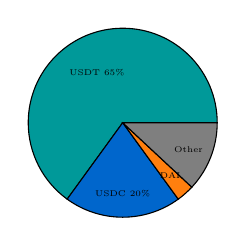
\begin{tikzpicture}[scale=0.6, transform shape]
% Pie chart style
\draw[fill=dfteal] (0,0) -- (0:2) arc (0:234:2) -- cycle;
\draw[fill=dfblue] (0,0) -- (234:2) arc (234:306:2) -- cycle;
\draw[fill=dforange] (0,0) -- (306:2) arc (306:317:2) -- cycle;
\draw[fill=dfgray] (0,0) -- (317:2) arc (317:360:2) -- cycle;

% Labels
\node[font=\tiny] at (117:1.2) {USDT 65\%};
\node[font=\tiny] at (270:1.5) {USDC 20\%};
\node[font=\tiny] at (312:1.5) {DAI};
\node[font=\tiny] at (338:1.5) {Other};
\end{tikzpicture}

\vspace{5mm}
\textbf{Growth Drivers:}
\begin{itemize}
\item Cross-border payments
\item DeFi activity
\item Emerging market adoption
\end{itemize}
\end{column}
\end{columns}
\end{frame}

% =============================================================================
% Frame 25: Hands-On Exercise I
% =============================================================================
\begin{frame}{Hands-On: NB10 --- Stablecoin Stability Analysis}
\begin{center}
\textbf{\Large Analyzing Peg Stability and De-Peg Events}
\end{center}

\vspace{5mm}
\textbf{In the Colab notebook (NB10), you will:}
\begin{enumerate}
\item Compare stability metrics across stablecoin types
\item Simulate crypto-collateralized stablecoin behavior
\item Model liquidation cascades under stress conditions
\item Analyze the Terra/UST death spiral dynamics
\item Calculate stability scores for different designs
\end{enumerate}

\vspace{5mm}
\begin{block}{Access the Notebook}
\texttt{day\_04/notebooks/NB10\_Stablecoin\_Analysis.ipynb}

\vspace{2mm}
\footnotesize Or scan QR code / click link provided
\end{block}

\bottomnote{Time: 20-25 minutes for guided exploration}
\end{frame}

% =============================================================================
% Frame 26: Hands-On Exercise II
% =============================================================================
\begin{frame}{NB10: Key Analysis Tasks}
\begin{columns}[T]
\begin{column}{0.48\textwidth}
\textbf{Part 1: Stability Metrics}
\begin{itemize}
\item Generate synthetic price data
\item Calculate mean/max deviation
\item Measure time within bands
\item Compare across types
\end{itemize}

\vspace{3mm}
\textbf{Part 2: Collateral Simulation}
\begin{itemize}
\item Build a DAI-like system
\item Open vaults with collateral
\item Simulate price decline
\item Observe liquidations
\end{itemize}
\end{column}

\begin{column}{0.48\textwidth}
\textbf{Part 3: Cascade Analysis}
\begin{itemize}
\item Model liquidation cascades
\item Vary market depth parameters
\item Observe feedback effects
\end{itemize}

\vspace{3mm}
\textbf{Part 4: Death Spiral}
\begin{itemize}
\item Simulate algorithmic collapse
\item Understand reflexivity
\item Identify warning signs
\end{itemize}

\vspace{3mm}
\begin{alertblock}{Key Takeaway}
Hands-on simulation reveals risks that theory alone cannot convey.
\end{alertblock}
\end{column}
\end{columns}
\end{frame}

% =============================================================================
% Frame 27: Discussion - Choosing a Stablecoin
% =============================================================================
\begin{frame}{Discussion: Which Stablecoin Should You Use?}
\begin{columns}[T]
\begin{column}{0.48\textwidth}
\textbf{For Maximum Safety:}
\begin{itemize}
\item USDC (fiat-backed, audited)
\item Accept centralization risk
\item Best for: Large holdings, institutions
\end{itemize}

\vspace{3mm}
\textbf{For Decentralization:}
\begin{itemize}
\item DAI (crypto-collateralized)
\item Accept capital inefficiency
\item Best for: DeFi natives, censorship concerns
\end{itemize}

\vspace{3mm}
\textbf{For Higher Yield:}
\begin{itemize}
\item Be extremely cautious
\item Understand yield source
\item Best for: Experienced users only
\end{itemize}
\end{column}

\begin{column}{0.48\textwidth}
\textbf{Questions to Ask:}
\begin{enumerate}
\item What backs the stablecoin?
\item Who can freeze my funds?
\item What happens if issuer fails?
\item How transparent are reserves?
\item What's the track record?
\end{enumerate}

\vspace{3mm}
\begin{block}{Portfolio Approach}
Many sophisticated users hold multiple stablecoins to diversify risk:
\begin{itemize}
\item 50\% USDC (safety)
\item 30\% DAI (decentralization)
\item 20\% other (diversification)
\end{itemize}
\end{block}
\end{column}
\end{columns}
\end{frame}

% =============================================================================
% Frame 28: Discussion - Systemic Risk
% =============================================================================
\begin{frame}{Discussion: Stablecoins as Systemic Risk?}
\begin{columns}[T]
\begin{column}{0.48\textwidth}
\textbf{Why Regulators Worry:}
\begin{itemize}
\item \$170B+ in circulation
\item Critical DeFi infrastructure
\item Bank-like without banking rules
\item Potential money laundering
\item Consumer protection gaps
\item ``Too big to fail'' concerns
\end{itemize}

\vspace{3mm}
\textbf{Historical Parallels:}
\begin{itemize}
\item Money market funds (2008)
\item Bank runs (pre-FDIC)
\item Currency crises
\end{itemize}
\end{column}

\begin{column}{0.48\textwidth}
\textbf{Counterarguments:}
\begin{itemize}
\item More transparent than banks
\item Real-time reserve verification
\item Market-based discipline
\item Innovation benefits
\end{itemize}

\vspace{3mm}
\begin{alertblock}{The Core Tension}
Should stablecoins be regulated like banks?
\begin{itemize}
\item Yes: Same risks, same rules
\item No: Different technology, different approach
\item Hybrid: Risk-based regulation
\end{itemize}
\end{alertblock}
\end{column}
\end{columns}
\end{frame}

% =============================================================================
% Frame 29: Stablecoin Regulation Overview
% =============================================================================
\begin{frame}{Stablecoin Regulation}
\begin{columns}[T]
\begin{column}{0.48\textwidth}
\textbf{Why Regulators Care:}
\begin{itemize}
\item Systemic risk (too big to fail?)
\item Consumer protection
\item Money laundering concerns
\item Monetary policy implications
\item Bank-like activities
\end{itemize}

\vspace{0.3cm}
\textbf{Regulatory Developments:}
\begin{itemize}
\item EU: MiCA framework (2024)
\item US: Congressional debate ongoing
\item Singapore: Clear framework
\item China: Banned
\end{itemize}
\end{column}

\begin{column}{0.48\textwidth}
\begin{block}{Key Requirements Emerging}
\begin{itemize}
\item 1:1 reserve backing
\item Regular audits/attestations
\item Redemption guarantees
\item Segregated reserves
\item Licensing requirements
\end{itemize}
\end{block}

\vspace{0.3cm}
\textbf{Impact on Market:}
\begin{itemize}
\item USDC: Embracing regulation
\item USDT: Offshore strategy
\item DAI: Decentralization defense
\end{itemize}
\end{column}
\end{columns}
\end{frame}

% =============================================================================
% Frame 30: MiCA and Future Regulation
% =============================================================================
\begin{frame}{MiCA: Europe's Stablecoin Framework}
\begin{columns}[T]
\begin{column}{0.55\textwidth}
\textbf{Markets in Crypto-Assets (MiCA):}
\begin{itemize}
\item First comprehensive crypto regulation
\item Effective 2024 for stablecoins
\item Applies to all EU member states
\end{itemize}

\vspace{3mm}
\textbf{Key Stablecoin Requirements:}
\begin{enumerate}
\item \textbf{Authorization}: Must be licensed
\item \textbf{Reserves}: 1:1 backing required
\item \textbf{Segregation}: Customer funds protected
\item \textbf{Redemption}: On-demand at par value
\item \textbf{Volume limits}: Caps on non-euro stablecoins
\end{enumerate}
\end{column}

\begin{column}{0.42\textwidth}
\textbf{Two Categories:}
\begin{itemize}
\item \textbf{EMT}: E-money tokens (single fiat)
\item \textbf{ART}: Asset-referenced tokens (baskets)
\end{itemize}

\vspace{3mm}
\begin{alertblock}{Impact}
\begin{itemize}
\item USDT delisted from some EU exchanges
\item USDC becoming ``compliant choice''
\item Euro stablecoins emerging
\item Algorithmic stablecoins effectively banned
\end{itemize}
\end{alertblock}
\end{column}
\end{columns}
\end{frame}

% =============================================================================
% Frame 31: Executive Summary
% =============================================================================
\begin{frame}{Executive Summary}
\begin{center}
\textbf{\Large Key Takeaways from Topic 4.3}
\end{center}

\vspace{3mm}
\begin{enumerate}
\item \textbf{Three design types} with different trade-offs\\
\footnotesize Fiat-backed (stable, centralized), Crypto-collateralized (decentralized, inefficient), Algorithmic (efficient, risky)

\item \textbf{The Stablecoin Trilemma constrains design}\\
\footnotesize Can only optimize two of: Decentralization, Stability, Capital Efficiency

\item \textbf{Peg mechanisms rely on arbitrage and trust}\\
\footnotesize Without reliable redemption, pegs can break catastrophically

\item \textbf{Terra/UST proved algorithmic stability is fragile}\\
\footnotesize Death spirals destroy value rapidly when confidence breaks

\item \textbf{Heavy regulatory scrutiny is coming}\\
\footnotesize MiCA in EU, pending legislation in US, global coordination
\end{enumerate}

\vspace{3mm}
\begin{block}{The Big Idea}
Stablecoins are the critical bridge between crypto and traditional finance, but each design involves fundamental trust trade-offs.
\end{block}
\end{frame}

% =============================================================================
% Frame 32: Concept Map
% =============================================================================
\begin{frame}{Concept Map: Stablecoin Ecosystem}
\begin{center}
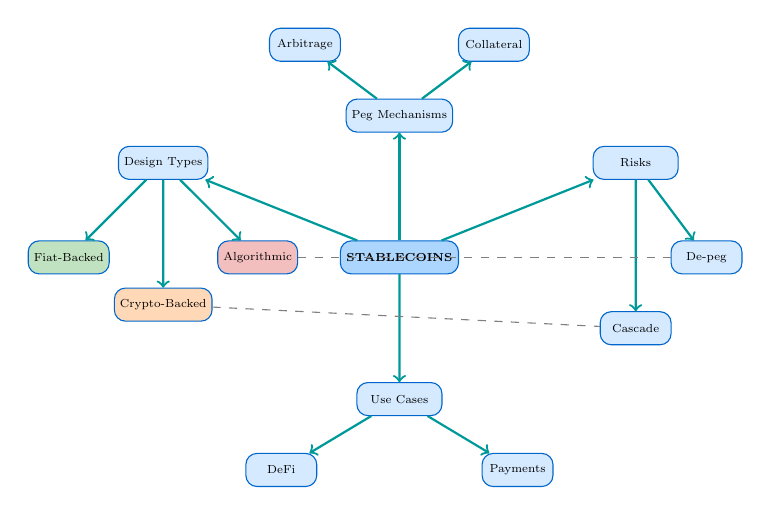
\begin{tikzpicture}[scale=0.6, transform shape,
    concept/.style={rectangle, rounded corners, draw=dfblue, fill=dflightblue4, minimum width=1.8cm, minimum height=0.7cm, font=\scriptsize},
    relationship/.style={->, thick, dfteal}]

% Central concept
\node[concept, fill=dflightblue2, minimum width=2.5cm] (stable) at (0,0) {\textbf{STABLECOINS}};

% Main branches
\node[concept] (types) at (-5,2) {Design Types};
\node[concept] (mechanisms) at (0,3) {Peg Mechanisms};
\node[concept] (risks) at (5,2) {Risks};
\node[concept] (uses) at (0,-3) {Use Cases};

% Types
\node[concept, minimum width=1.5cm, fill=dfgreen!30] (fiat) at (-7,0) {Fiat-Backed};
\node[concept, minimum width=1.5cm, fill=dforange!30] (crypto) at (-5,-1) {Crypto-Backed};
\node[concept, minimum width=1.5cm, fill=dfred!30] (algo) at (-3,0) {Algorithmic};

% Mechanisms
\node[concept, minimum width=1.5cm] (arb) at (-2,4.5) {Arbitrage};
\node[concept, minimum width=1.5cm] (collat) at (2,4.5) {Collateral};

% Risks
\node[concept, minimum width=1.5cm] (depeg) at (6.5,0) {De-peg};
\node[concept, minimum width=1.5cm] (cascade) at (5,-1.5) {Cascade};

% Uses
\node[concept, minimum width=1.5cm] (defi) at (-2.5,-4.5) {DeFi};
\node[concept, minimum width=1.5cm] (payments) at (2.5,-4.5) {Payments};

% Connections
\draw[relationship] (stable) -- (types);
\draw[relationship] (stable) -- (mechanisms);
\draw[relationship] (stable) -- (risks);
\draw[relationship] (stable) -- (uses);

\draw[relationship] (types) -- (fiat);
\draw[relationship] (types) -- (crypto);
\draw[relationship] (types) -- (algo);

\draw[relationship] (mechanisms) -- (arb);
\draw[relationship] (mechanisms) -- (collat);

\draw[relationship] (risks) -- (depeg);
\draw[relationship] (risks) -- (cascade);

\draw[relationship] (uses) -- (defi);
\draw[relationship] (uses) -- (payments);

% Cross-connections
\draw[dashed, dfgray] (algo) -- (depeg);
\draw[dashed, dfgray] (crypto) -- (cascade);
\end{tikzpicture}
\end{center}
\end{frame}

% =============================================================================
% Frame 33: Key Terms & Definitions I
% =============================================================================
\begin{frame}{Key Terms \& Definitions (I)}
\begin{description}
\item[Stablecoin] A cryptocurrency designed to maintain a stable value relative to a reference asset (typically \$1 USD).

\item[Peg] The target price a stablecoin aims to maintain, typically \$1.00.

\item[De-peg] When a stablecoin's market price deviates significantly from its target peg.

\item[Fiat-Backed Stablecoin] A stablecoin backed 1:1 by fiat currency reserves held by a centralized issuer (e.g., USDC, USDT).

\item[Collateralization Ratio] The ratio of collateral value to debt; crypto-backed stablecoins typically require 150\%+ collateralization.
\end{description}
\end{frame}

% =============================================================================
% Frame 34: Key Terms & Definitions II
% =============================================================================
\begin{frame}{Key Terms \& Definitions (II)}
\begin{description}
\item[Crypto-Collateralized Stablecoin] A stablecoin backed by over-collateralized cryptocurrency locked in smart contracts (e.g., DAI).

\item[Algorithmic Stablecoin] A stablecoin that maintains its peg through algorithmic supply adjustments rather than collateral backing.

\item[Liquidation] The forced sale of collateral when a vault's collateralization ratio falls below the minimum threshold.

\item[Death Spiral] A reflexive feedback loop where falling prices trigger mechanisms that cause further price declines.

\item[Stablecoin Trilemma] The impossibility of simultaneously achieving full decentralization, perfect stability, and high capital efficiency.

\item[Attestation] An independent accounting report verifying stablecoin reserves (less rigorous than a full audit).
\end{description}
\end{frame}

% =============================================================================
% Frame 35: Common Misconceptions
% =============================================================================
\begin{frame}{Common Misconceptions}
\begin{columns}[T]
\begin{column}{0.48\textwidth}
\textbf{\textcolor{dfred}{Misconception}}

\vspace{2mm}
``Stablecoins are stable''

\vspace{5mm}
``Fiat-backed means risk-free''

\vspace{5mm}
``Algorithmic = decentralized = good''

\vspace{5mm}
``Higher yield = better stablecoin''
\end{column}

\begin{column}{0.48\textwidth}
\textbf{\textcolor{dfgreen}{Reality}}

\vspace{2mm}
Stablecoins \textit{target} stability but can de-peg, especially during market stress

\vspace{2mm}
Fiat-backed coins carry counterparty, banking, and regulatory risks (see SVB crisis)

\vspace{2mm}
Algorithmic designs have proven fragile; decentralization alone doesn't ensure stability

\vspace{2mm}
Unsustainable yield is often a warning sign of hidden risks (see Anchor/UST)
\end{column}
\end{columns}

\vspace{5mm}
\begin{alertblock}{Critical Thinking}
Always ask: What backs this stablecoin? Who can freeze it? What happens in a crisis?
\end{alertblock}
\end{frame}

% =============================================================================
% Frame 36: Self-Assessment Question 1
% =============================================================================
\begin{frame}{Self-Assessment: Question 1}
\begin{block}{Question}
Which of the following is NOT a characteristic of fiat-backed stablecoins like USDC?
\end{block}

\vspace{3mm}
\begin{enumerate}[A.]
\item 1:1 backing by USD or USD-equivalent reserves
\item Centralized issuer that can freeze addresses
\item Over-collateralization requirement of 150\%+
\item Regular attestation reports on reserve holdings
\end{enumerate}

\vspace{5mm}
\pause
\textbf{Answer: C}

\vspace{2mm}
\textbf{Explanation:} Fiat-backed stablecoins use 1:1 backing (100\% collateralization), not over-collateralization. The 150\%+ over-collateralization requirement is characteristic of \textit{crypto-collateralized} stablecoins like DAI, which need extra buffer due to collateral volatility.
\end{frame}

% =============================================================================
% Frame 37: Self-Assessment Questions 2-3
% =============================================================================
\begin{frame}{Self-Assessment: Questions 2-3}
\begin{block}{Question 2 (from Quiz)}
What is the Stablecoin Trilemma?
\end{block}
\textbf{Answer:} The impossibility of simultaneously achieving \textbf{decentralization}, \textbf{stability}, and \textbf{capital efficiency}. Every stablecoin design must compromise on at least one dimension.

\vspace{5mm}
\begin{block}{Question 3 (from Quiz)}
Why did the Terra/UST algorithmic stablecoin collapse?
\end{block}
\textbf{Answer:} UST relied on a reflexive mint/burn mechanism with LUNA. When confidence broke, mass redemptions crashed LUNA's price, making it impossible to absorb UST selling pressure. This created a \textbf{death spiral}---a feedback loop where falling prices trigger mechanisms that cause further price declines.

\vspace{3mm}
\textbf{Key Lesson:} When the peg mechanism depends on confidence in the peg, the system is vulnerable to self-fulfilling collapse.
\end{frame}

% =============================================================================
% Frame 38: What's Next - Preview T4.4
% =============================================================================
\begin{frame}{What's Next: Topic 4.4}
\begin{center}
\textbf{\Large Preview: Tokenization of Real-World Assets}
\end{center}

\vspace{5mm}
\textbf{In Topic 4.4, we'll explore:}
\begin{itemize}
\item \textbf{Real-World Asset (RWA) tokenization}---putting stocks, bonds, real estate on-chain
\item \textbf{Central Bank Digital Currencies (CBDCs)}---digital government money
\item \textbf{Security tokens}---regulated digital securities
\item \textbf{The convergence} of traditional and decentralized finance
\end{itemize}

\vspace{5mm}
\begin{block}{Connection}
Topic 4.3 covered stablecoins as the first bridge between TradFi and crypto.\\
Topic 4.4 extends this to tokenizing \textit{all} real-world assets.
\end{block}

\vspace{3mm}
\textbf{Preparation:} Consider how stablecoin mechanisms might apply to tokenized assets.
\end{frame}

% =============================================================================
% Frame 39: Resources
% =============================================================================
\begin{frame}{Resources for Further Learning}
\textbf{Essential Reading:}
\begin{itemize}
\item MakerDAO Documentation (DAI mechanics)
\item Circle USDC Transparency Reports
\item Terra Post-Mortem Analysis
\end{itemize}

\vspace{3mm}
\textbf{Online Resources:}
\begin{itemize}
\item Course notebook: \texttt{NB10\_Stablecoin\_Analysis.ipynb}
\item DeFiLlama Stablecoin Dashboard: \url{https://defillama.com/stablecoins}
\item The Block: Stablecoin Reports
\end{itemize}

\vspace{3mm}
\textbf{Academic References:}
\begin{itemize}
\item Klages-Mundt et al. ``Stablecoins 2.0'' (DeFi stability analysis)
\item BIS Reports on Stablecoins and Financial Stability
\end{itemize}

\vspace{3mm}
\begin{block}{Course Materials}
All slides and notebooks available on the course website.
\end{block}
\end{frame}

% =============================================================================
% Frame 40: Questions?
% =============================================================================
\begin{frame}{Questions?}
\begin{center}
\textbf{\LARGE Questions \& Discussion}

\vspace{10mm}
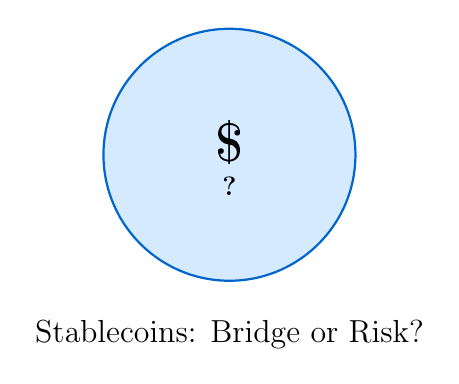
\begin{tikzpicture}[scale=0.8, transform shape]
% Question mark with stablecoin theme
\draw[thick, dfblue, fill=dflightblue4] (0,0) circle (2cm);
\node at (0,0.2) {\Huge \textbf{\$}};
\node at (0,-0.5) {\large \textbf{?}};
\node[below] at (0,-2.5) {\Large Stablecoins: Bridge or Risk?};
\end{tikzpicture}

\vspace{10mm}
\textbf{Contact:} joerg.osterrieder@gmail.com

\vspace{3mm}
\textbf{Next Topic:} T4.4 --- Tokenization and CBDCs
\end{center}
\end{frame}

\end{document}
